% (The MIT License)
%
% Copyright (c) 2023 Yegor Bugayenko
%
% Permission is hereby granted, free of charge, to any person obtaining a copy
% of this software and associated documentation files (the 'Software'), to deal
% in the Software without restriction, including without limitation the rights
% to use, copy, modify, merge, publish, distribute, sublicense, and/or sell
% copies of the Software, and to permit persons to whom the Software is
% furnished to do so, subject to the following conditions:
%
% The above copyright notice and this permission notice shall be included in all
% copies or substantial portions of the Software.
%
% THE SOFTWARE IS PROVIDED 'AS IS', WITHOUT WARRANTY OF ANY KIND, EXPRESS OR
% IMPLIED, INCLUDING BUT NOT LIMITED TO THE WARRANTIES OF MERCHANTABILITY,
% FITNESS FOR A PARTICULAR PURPOSE AND NONINFRINGEMENT. IN NO EVENT SHALL THE
% AUTHORS OR COPYRIGHT HOLDERS BE LIABLE FOR ANY CLAIM, DAMAGES OR OTHER
% LIABILITY, WHETHER IN AN ACTION OF CONTRACT, TORT OR OTHERWISE, ARISING FROM,
% OUT OF OR IN CONNECTION WITH THE SOFTWARE OR THE USE OR OTHER DEALINGS IN THE
% SOFTWARE.

\documentclass{article}
\usepackage{../sqm}
\newcommand*\thetitle{Code Churn}
\begin{document}

\plush{\sqmTitlePage{13}}

\pitch{\pptBanner{History of Version Control Systems}
\begin{itemize}\setlength\itemsep{0pt}
  \item The Librarian by ADR: 1969
  \item Panvalet by Computer Associates: 1969
  \item SCCS by Bell Labs: 1973
  \item RCS by GNU: 1982
  \item CVS: 1986
  \item ClearCase by IBM: 1992
  \item Apache Subversion: 2000
  \item Mercurial: 2005
  \item Git: 2005
\end{itemize}}

\pitch{\pptQuote{sebastian-elbaum.jpg}{We can measure the increase or decrease in system complexity as measured by a selected metric, \emph{code delta}, or we can measure the total amount of \emph{change} the system has undergone between builds, \emph{code churn}.}{\textit{Code Churn: A Measure for Estimating the Impact of Code Change}, \emph{Sebastian G. Elbaum} and John C. Munson, Proceedings of the International Conference on Software Maintenance (ICSM), 1998}}

\pptBanner{Motivating Example}
\begin{pptWide}{3}
Commit \#1:\par
0\par
{\small\begin{ffcode}
class Book
  private final int id;
  public Book(int it)
    this.id = i;
\end{ffcode}
}
\par\columnbreak\par
Commit \#2:\par
\textcolor{green}{+5}\par
{\small\begin{ffcode}
class Book
  private int id;
  public Book(int it)
    this.id = i;
  public int getId()
    return this.id;
  private int setId(int i)
    this.id = i;
\end{ffcode}
}
\par\columnbreak\par
Commit \#3:\par
\textcolor{green}{+2} / \textcolor{red}{-2}\par
{\small\begin{ffcode}
final class Book
  private final int id;
  public Book(int it)
    this.id = i;
  public int getId()
    return this.id;
\end{ffcode}
}
\end{pptWide}
Delta: \textcolor{green}{+3} / 0, Churn: \textcolor{green}{+7} / \textcolor{red}{-2}
\plush{}

\pptBanner{Code Delta vs. Code Churn}
\begin{multicols}{2}
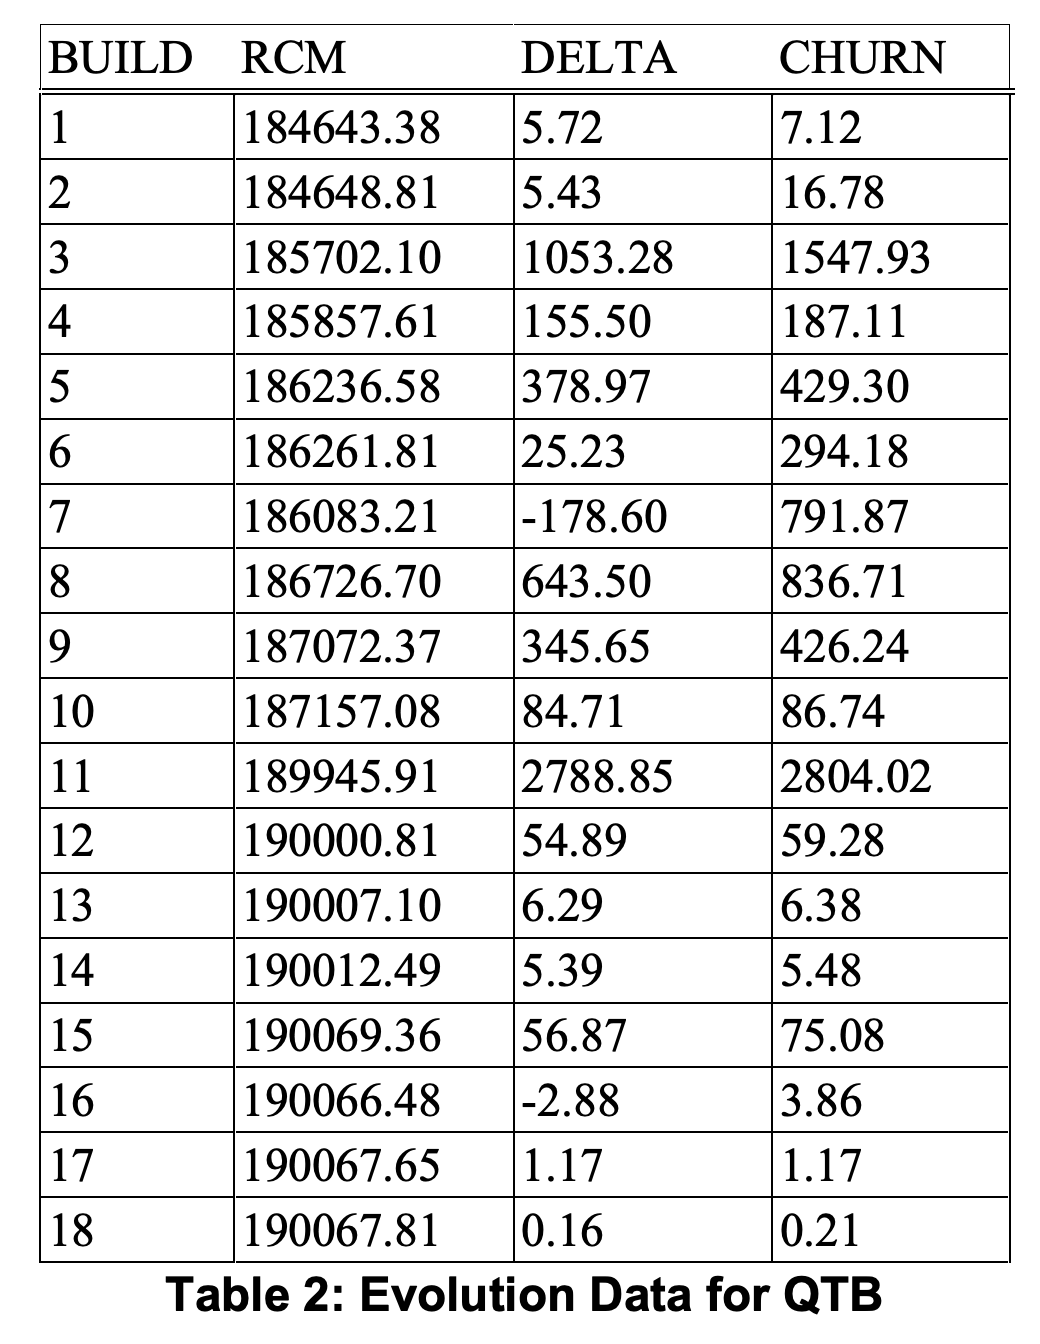
\includegraphics[width=.7\columnwidth]{qtb.png}
\par\columnbreak\par
``A limitation of measuring code deltas is that it
doesn’t give an indicator as to how much change the
system has undergone. If several
software modules are removed and are replaced by
modules of roughly equivalent complexity, the code
delta for the system will be close to zero.''
\par
{\scriptsize Source: \textit{Code Churn: A Measure for Estimating the Impact of Code Change}, Sebastian G. Elbaum et al., ICSM, 1998\par}
\end{multicols}
\plush{}

\pitch{\pptQuote{nachiappan-nagappan.jpg}{Our case study provides strong support for the following conclusion: increase in relative code churn measures is accompanied by an increase in system \emph{defect density}.}{\textit{Use of Relative Code Churn Measures to Predict System Defect Density}, \emph{Nachiappan Nagappan} and Thomas Ball, Proceedings of the International Conference on Software Engineering (ICSE), 2005}}

\pitch{\pptQuote{rudolf-ferenc.jpg}{We can conclude that committing files with higher cumulative code churn values (i.e. those of longer change history) is more likely to result in negative maintainability change.}{\textit{Cumulative Code Churn: Impact on Maintainability}, Csaba Farag{\'o}, P{\'e}ter Heged{\H{u}}s, \emph{Rudolf Ferenc}, Proceedings of the International Working Conference on Source Code Analysis and Manipulation (SCAM), 2015}}

\pitch{\pptQuote{tobias-olsson.jpg}{Non-normal code churn can be a tangible and measurable \emph{effect} of architectural violations in source code. However, more research is needed to better understand this connection, e.g., if violations are the \emph{cause}, the size of the effect, the cost of refactoring, and whether it is generalizable to other system.}{\textit{The Relationship of Code Churn and Architectural Violations in
the Open Source Software JabRef}, Tobias Olsson, Morgan Ericsson, Anna Wingkvist, Proceedings of the 11th European Conference on Software Architecture: Companion Proceedings, 2017}}

\pitch{\pptBanner{CodeClimate.com Interpretation of Code Churn}
\begin{multicols}{2}
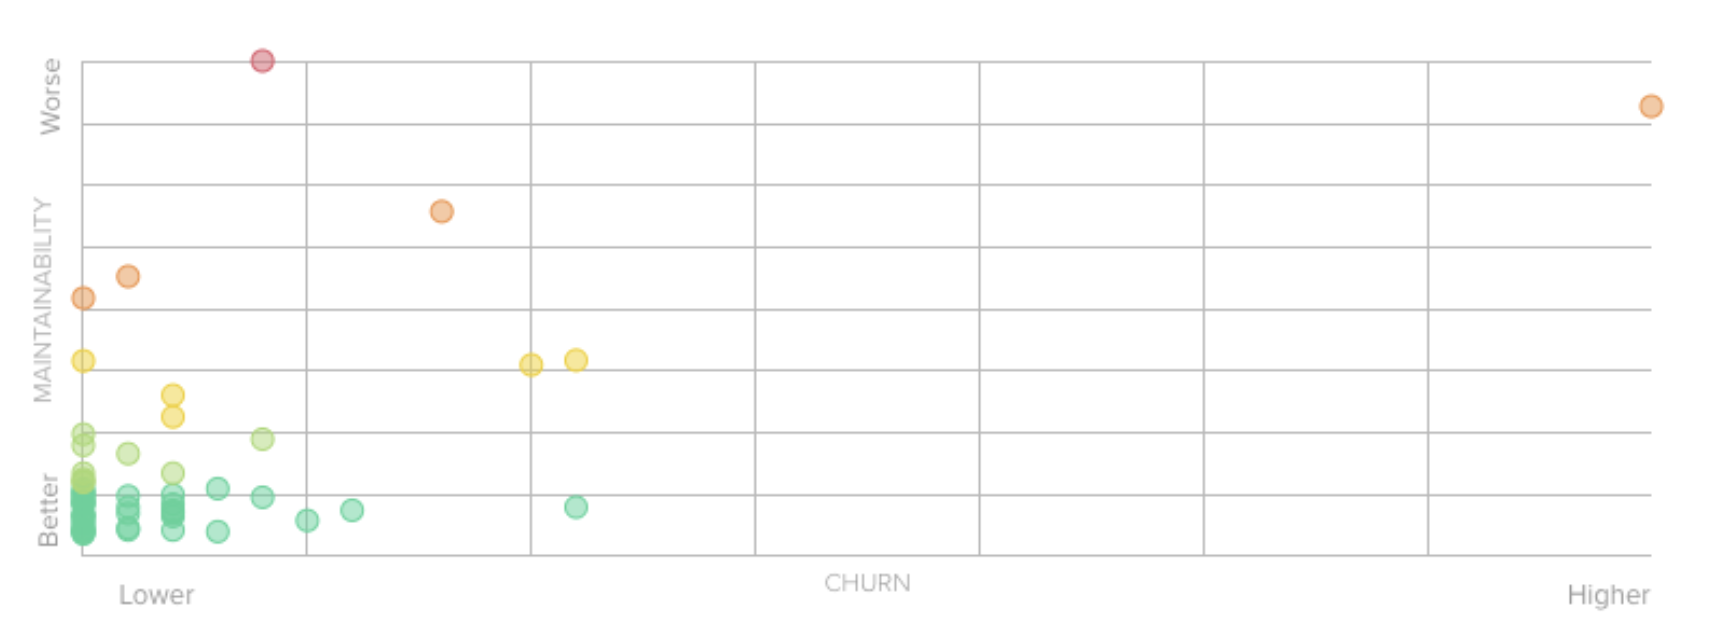
\includegraphics[width=.98\columnwidth]{codeclimate.png}
\par\columnbreak\par
``When we have finished analyzing your default branch, you will see churn metrics for the files in your repository. This churn metric is approximately the \emph{number of times a file has changed} in the last 90 days, calculated by counting the number of distinct versions of that file across commits from that time.''\par
{\scriptsize Source: \href{https://docs.codeclimate.com/docs/churn}{their blog}\par}
\end{multicols}}

\pptBanner{HitsOfCode.com}
\begin{multicols}{2}
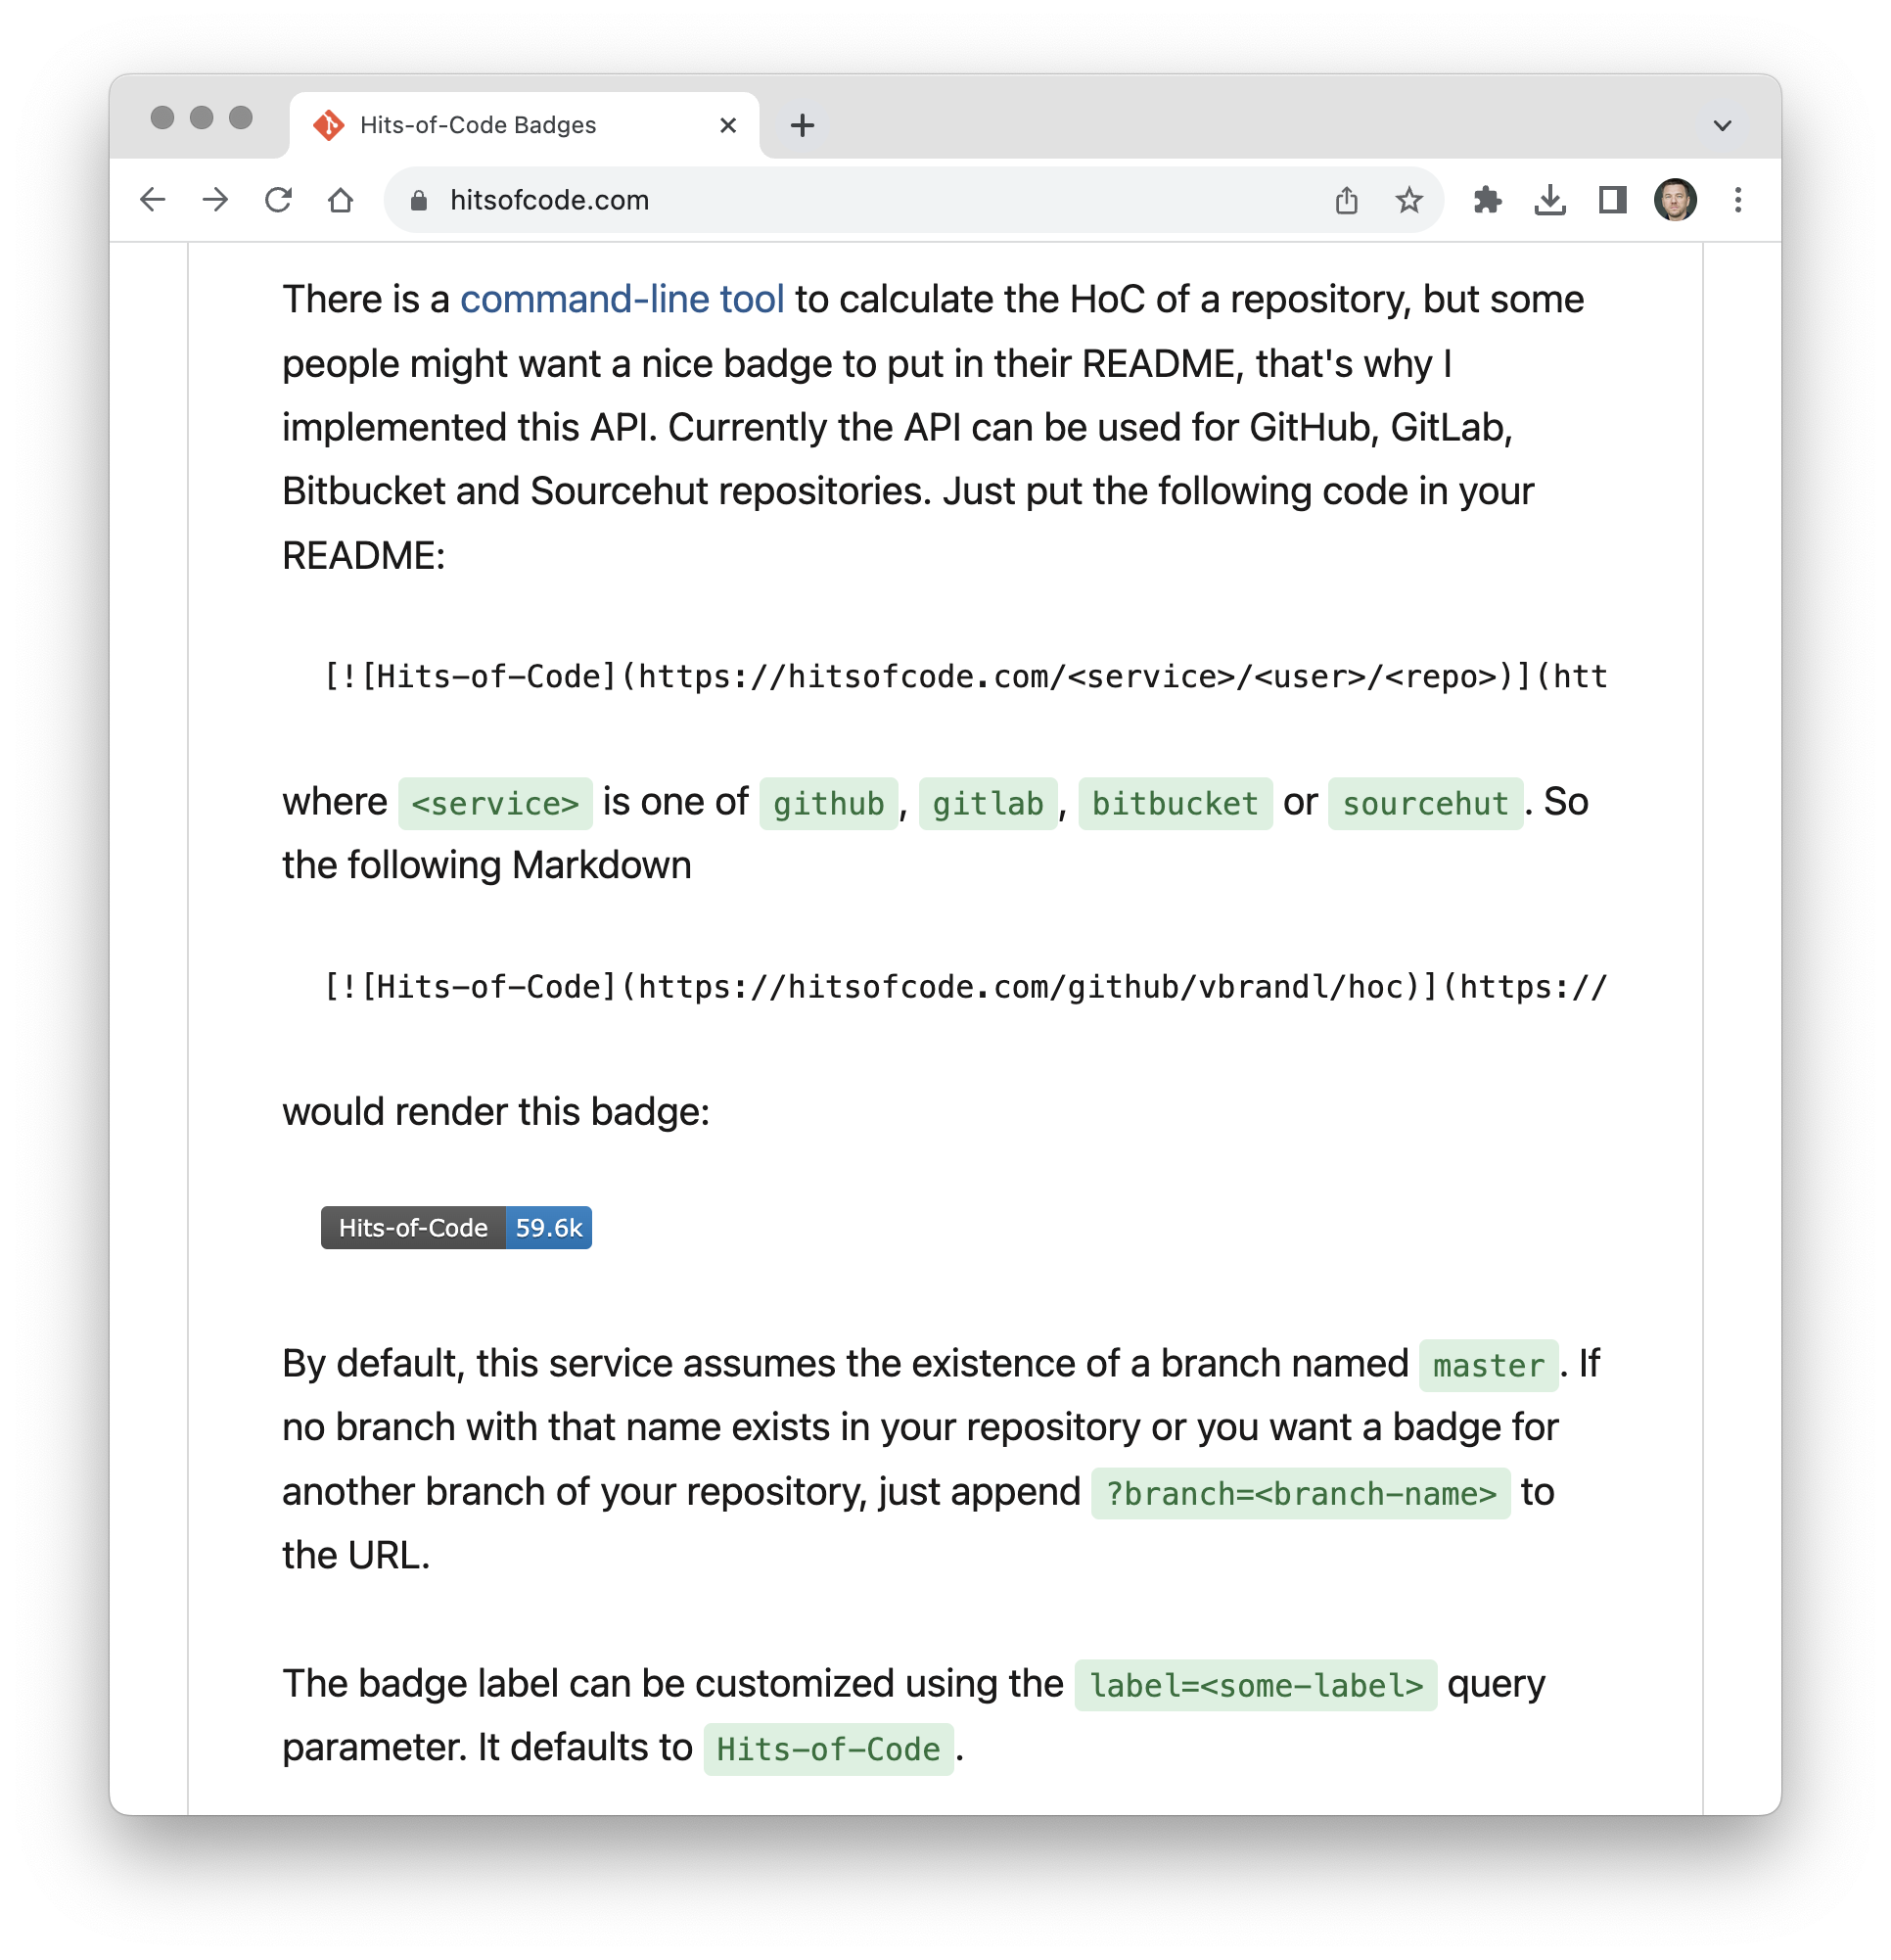
\includegraphics[width=.9\columnwidth]{hitsofcode.png}
\par\columnbreak\par
Created by \href{https://www.vbrandl.net/}{Valentin Brandl} (@vbrandl)
and inspired by the blog post of mine:
\href{https://www.yegor256.com/2014/11/14/hits-of-code.html}{Hits-of-Code Instead of SLoC} (2014)
\end{multicols}
\plush{}

\plush{
  \pptBanner{Read this:}\par
  \small
  \textit{Code Churn: A Measure for Estimating the Impact of Code Change},
    Sebastian G. Elbaum and John C. Munson,
    Proceedings of the International Conference on Software Maintenance (ICSM), 1998\par
  \href{https://www.yegor256.com/2014/11/14/hits-of-code.html}{Hits-of-Code Instead of SLoC} (2014) \par
}

\end{document}
